

\section{Classement par mesure d'importance}


\begin{frame}{PageRank\,: importance déduite du graphe des documents}

Dans le cas du Web (et quelques autres systèmes), les documents
sont liés par des hyperliens.

\vfill

La structure de la collection est donc celle d'un \alert{graphe orienté}.

\vfill

\begin{block}{Intuition}
Un document vers lequel convergent beaucoup de chemins est 
un document \alert{important}.
\end{block}

\vspace{.5cm}

En combinant avec des mesures de pertinence (tf/idf), on obtient un moyen d'améliorer
le classement.

\end{frame}

\begin{frame}
\frametitle{PageRank\,: définition et  exemples}

\begin{block}{Définition}
L'indicateur \emph{PageRank} (PR) d'une page  $p_i$ est la \alert{probabilité} 
qu'un utilisateur suivant les liens de manière aléatoire arrive sur $P_i$.
\end{block}

 
 \figSlideWithSize{pagerank-basic}{11cm}
 
 À gauche\,: la probabilité d'arriver en $A$ en \alert{une} étape est $PR(A) = PR(B) + PR(C) + PR (D)$
 
  \vfill
 À droite\,?
 \vfill
 Au départ, chaque page a un PR de 0,25.  Quel est le PR après une itération\,? Et après deux\,?

 
\end{frame}

\begin{frame}
\frametitle{Un exemple plus complet}


\centering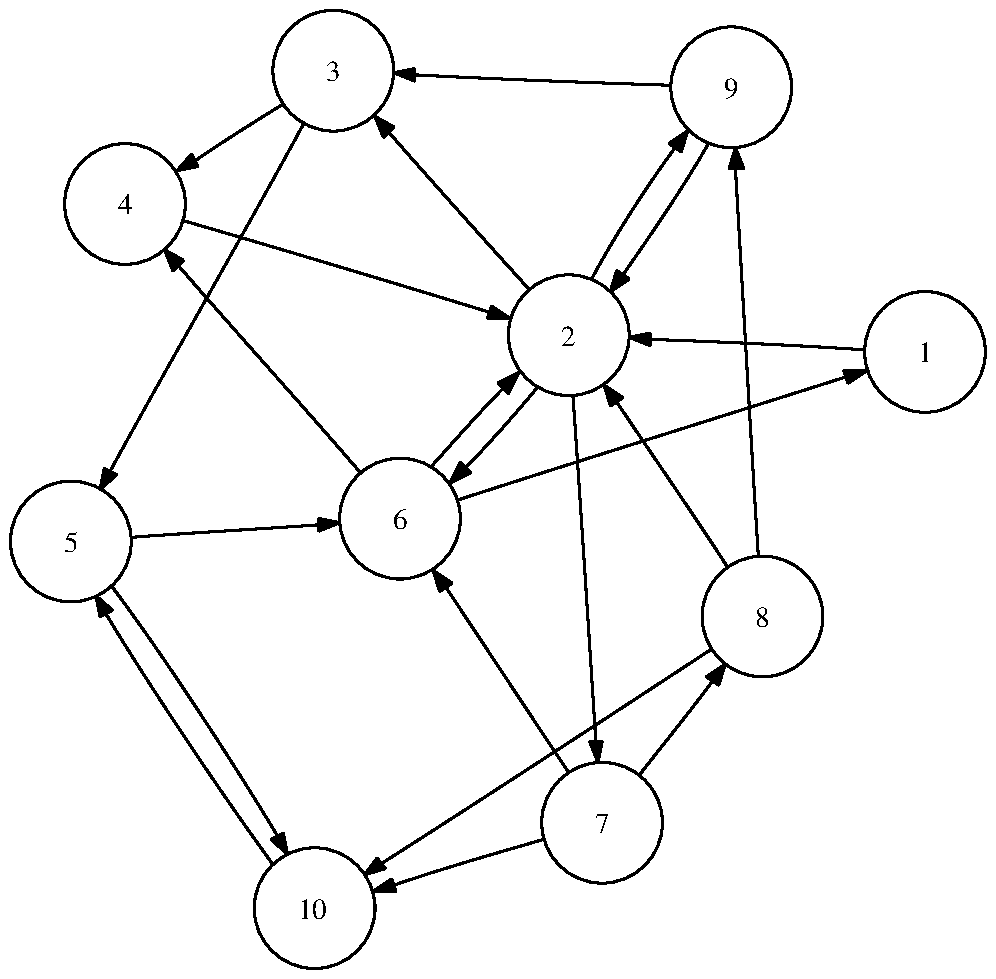
\includegraphics[width=.7\linewidth]{images/graph}

\end{frame}

\begin{frame}
\frametitle{On construit une \alert{matrice de transition}}

\[\begin{cases} g_{ij}=0&\text{s'il n'y a pas de lien entre les pages  $i$ et
$j$;}\\ g_{ij}=\frac{1}{n_i}&\text{sinon, $n_i$ étant le nombre de liens sortant de la page $i$.}\end{cases}\]


\[
G=\begin{pmatrix}
0&1&0&0&0&0&0&0&0&0\\
0&0&\frac 1 4&0&0&\frac 1 4&\frac 1 4&0&\frac 1 4&0\\
0&0&0&\frac 1 2&\frac 1 2&0&0&0&0&0\\
0&1&0&0&0&0&0&0&0&0\\
0&0&0&0&0&\frac 1 2&0&0&0&\frac 1 2\\
\frac 1 3&\frac 1 3&0&\frac 1 3&0&0&0&0&0&0\\
0&0&0&0&0&\frac 1 3&0&\frac 1 3&0&\frac 1 3\\
0&\frac 1 3&0&0&0&0&0&0&\frac 1 3&\frac 1 3\\
0&\frac 1 2&\frac 1 2&0&0&0&0&0&0&0\\
0&0&0&0&1&0&0&0&0&0\\
\end{pmatrix}
\]
\end{frame}

\begin{frame}{Calcul du PageRank, pas à pas}

Je veux calculer la probablité d'être en $N_2$ à
l'étape $e$. J'ai besoin\,:

\begin{itemize}
  \item de la probabilité d'être sur chaque n{\oe}ud $N_i$ à l'étape  $e-1$
  
     $\Rightarrow$ c'est le vecteur des PageRank, appelons-le $v$.
     
  \item de la probabilité d'arriver au n{\oe}ud $N_2$ venant du n{\oe}ud $N_i$ 
  
   $\Rightarrow$ c'est la seconde \alert{colonne} de la matrice.    
\end{itemize}

Allons-y. Au départ, le vecteur des PageRank est uniforme

 $$v= [0.1, 0.1, 0.1, 0.1, 0.1, 0.1, 0.1, 0.1, 0.1, 0.1]$$
 
La seconde colonne de la matrice, \alert{transposée} est\,:

 $$C_2= [1, 0, 0, 1, 0, 1/3, 0, 1/3, 1/2, 0]$$ 
 
Ce qui donne la probabilité d'arriver en $N_2$ à la première itération

$$0.1 \times 1 + 0.1 \times 1 + 0.1 \times 1/3 + 0.1 \times 1/3+ 0.1 \times 1/2 = 0.317$$

Interprétation\,: j'ai 10\% de chances d'être en $N_1$, 100\% de chances, étant en $N_1$, d'aller en $N_2$, etc.
\end{frame}

\begin{frame}{Calcul du PageRank, généralisé}

On effectue le calcul précédent pour tous les n{\oe}uds, et autant de fois que nécessaire.
\begin{itemize}
  \item On construit par itérations un vecteur contenant l'indicateur PR de chaque page du  graphe.

     Appelons-le $v$\,; il contient autant de coordonnées que de pages du Web...
     
     \item $v$ est initialisé avec une distribution uniforme  ($v[i] = \frac{1}{|v|}$).

   Sur notre exemple, la valeur initiale est 1/10.

  \item À chaque itération, on ajuste $v$ on calculant la probabilité qu'un
  déplacement amène sur chaque n{\oe}ud.
  
  
   On multiplie le vecteur $v$ par la \alert{transposée} de $G$ (les colonnes
      donnent la probabilité d'\alert{arriver} sur un n{\oe}ud).

\end{itemize}


   On peut montrer qu'il y a \alert{convergence} du vecteur $v$ vers une limite.
   
   
\[\mathop{\mathsf{pr}}(i)=\left(\lim_{k\rightarrow+\infty}(G^T)^kv\right)_i \]

\end{frame}



\begin{frame}{Queques itérations PageRank}
\iterations{pr}
\end{frame}


\begin{comment}
\begin{frame}
\frametitle{Exercice}


 \figSlide{pagerank-basic}
 
Représenter la matrice de transition et appliquer PageRank.
\end{frame}
\end{comment}

\begin{frame}{Petite extension pratique}

Pour mieux modéliser le comportement d'un utilisateur, on s'autorise des
\alert{sauts} d'une page à une autre, sans qu'il y ait nécessairement de lien.

\vfill

À chaque étape, on prend en compte la possibilité d'un tel saut avec
une probabilité  $d$ ($1-d$: \alert{damping factor}). Ce qui donne\,:

\[
\mathop{\mathsf{pr}}(i)=\left(\lim_{k\rightarrow+\infty}((1-d)G^T+dU)^kv\right)_i
\] où $U$ est une matrice contenant $\frac{1}{N}$ dans chaque cellule.

\end{frame}
